% ------------------------------------------------------------------------------
% LaTeX Template: Presentation Slides
% This is LaTeX template is suitable for (technical) presentations
%
% Copyright: Marius Hofert, Markus Kohm (PracTeX)
% The idea of this template came from The PracTeX Journal 2010-2
% Date: April 2011
% ------------------------------------------------------------------------------

% ------------------------------------------------------------------------------
% Document
% ------------------------------------------------------------------------------
\documentclass[
	paper=128mm:96mm,	% like beamer
	fontsize=11pt,					% like beamer
	pagesize,							% write page size to dvi or pdf
	parskip=half-,					% paragraphs separated half a line, no marking of line endings
	numbers=noendperiod,	% removes points for special parts (e.g. appendix)
	captions=nooneline			% do not distinguish between one or more lines in captions
	]{scrartcl}							% KOMA script (article)

% Presentation tweaks	
\linespread{1.12} 				% enlarge line space

% Color
\usepackage{xcolor}			% color package; load before tocstyle

% Page structure
\usepackage{calc}				% working with lengths, counters etc.
\usepackage[
	includeheadfoot,%
	top=3.5mm,%
	bottom=3.5mm,%
	left=5.5mm,%
	right=5.5mm,%
	headsep=6.5mm,%
	footskip=8.5mm%
	]{geometry}						% set page layout parameters
\usepackage{scrpage2}		% package for page style with not only uppercase letters in the head 
\usepackage{titlesec}			% for reducing space between ((sub)sub)sections and text
\usepackage{tocstyle}			% for adjusting table of contents

% ------------------------------------------------------------------------------
% Document metadata
% Fill in your own stuff here
% ------------------------------------------------------------------------------
\newcommand*{\mytitle}{QuickDough: A Rapid FPGA Accelerator Design Framework 
Using Soft Coarse-Grained Reconfigurable Architecture Overlay}		% title
\newcommand*{\mytitleontitlepage}{\mytitle}	% title
\newcommand*{\myauthor}{Cheng Liu}				% name
\newcommand*{\mydate}{\today}						% date
\newcommand*{\myuni}{Department of Electrical and Electronic Engineering, HKU}			% university/department

% colors
\definecolor{mygreen}{RGB}{44,85,17}				% for emphasizing text (#2c5511)
\definecolor{myblue}{RGB}{34,31,217}					% for emphasizing text (#5d90c2)
\definecolor{mybrown}{RGB}{194,164,113}			% for emphasizing text (#c2a471)
\definecolor{myred}{RGB}{255,66,56}					% for emphasizing text (#cc7b76)
\newcommand*{\mygreen}[1]{\textcolor{mygreen}{#1}}
\newcommand*{\myblue}[1]{\textcolor{myblue}{#1}}
\newcommand*{\mybrown}[1]{\textcolor{mybrown}{#1}}
\newcommand*{\myred}[1]{\textcolor{myred}{#1}}

% ------------------------------------------------------------------------------
% Fonts
% ------------------------------------------------------------------------------
\usepackage[T1]{fontenc}	% for correct hyphenation and T1 encoding
\usepackage{lmodern}			% latin modern font

% Choose one of the following three fonts
%\usepackage{fourier}			% utopia
%\usepackage{charter}			% low-resolution roman font
\renewcommand{\familydefault}{\sfdefault}% sans serif

\usepackage[english]{babel}% for Brittish English
\usepackage{microtype}		% for character protrusion and font expansion (only with pdflatex)

% ------------------------------------------------------------------------------
% Misc
% ------------------------------------------------------------------------------ 
\usepackage{amsthm}			% theorem environments
\usepackage{bm}					% for bold math symbols
\usepackage{enumitem}		% for automatic numbering of new enumerate environments
\usepackage{graphicx}		% for including figures
\usepackage{tikz}				% sophisticated graphics package
\usepackage{tabularx}			% for special table environment (tabularx-table)
\usepackage{booktabs}		% for table layout
\usepackage[
	hypertexnames=false,		% for correct links (duplicate-error solution)
	setpagesize=false,			% to prevent change text-/paperformat for the document
	pdfborder={0 0 0},			% removes border around links
	pdfpagemode=FitH,% open pdf in full screen mode
   pdfstartview=Fit				% fit page to pdf viewer
]{hyperref}							% all links stay black and are thus invisible
\hypersetup{						% NOTE: If \myauthor or \mytitle contain non-us-ascii-chars you
           									% should not use them inside \hyperref.
  pdfauthor=\myauthor,%
  pdftitle=\mytitle%
}
\usepackage{lastpage}			% to denote last page in slide numbering

% ------------------------------------------------------------------------------
% Page Style
% ------------------------------------------------------------------------------
\pagestyle{scrheadings}		% activates pagestyle from scrpage2
\clearscrheadfoot					% clear head and foot of scrheadings and scrplain
\setkomafont{pageheadfoot}{\normalfont\color{black}\sffamily}% setting for page head and foot

% optical vertical centering of page contents
\makeatletter
\renewcommand*{\@textbottom}{\vskip \z@ \@plus 1fil}
\newcommand*{\@texttop}{\vskip \z@ \@plus .5fil}
\addtolength{\parskip}{\z@\@plus .25fil}% stetch parskip a lot
\makeatother

% spacings
\titlespacing{\section}{0mm}{0mm}{0mm}% space (left, before, after) between section and text
\titlespacing{\subsection}{0mm}{0mm}{-1mm}% space (left, before, after) between subsection and text
\titlespacing{\subsubsection}{0mm}{0mm}{-2mm}% space (left, before, after) between subsubsection and text
\setcounter{secnumdepth}{2}% add numbering down to subsection 

% foot
\newlength{\footheight}
\setlength{\footheight}{8mm}
\addtokomafont{pagefoot}{\footnotesize}% general setting for the foot
\setkomafont{pagenumber}{\color{black}}% setting for page foot
\ifoot{% foot left
	\hspace{-2mm}%
	\begin{tikzpicture}[remember picture,overlay]
		\node [xshift=\paperwidth/2,yshift=\footheight] at (current page.south west)[rectangle,fill,inner sep=0pt,minimum width=\paperwidth,minimum height=3pt,top color=mygreen,bottom color=mygreen]{};% bar 
	\end{tikzpicture}%
	\myauthor\ \raisebox{0.2mm}{$\bm{\vert}$}\ \myuni
}
\ofoot[\pagemark/\pageref{LastPage}\hspace{-2mm}]{% foot right
	\pagemark/\pageref{LastPage}\hspace{-2mm}}

% table of contents
\AtBeginDocument{\renewcaptionname{english}{\contentsname}{\large Outline}}% change name of toc
\makeatletter
\newtocstyle[noonewithdot]{nodotnopagenumber}{% define tocstyle without dots and page numbers
  \settocfeature{pagenumberbox}{\@gobble}%
}
\makeatother
\usetocstyle{nodotnopagenumber}

% theorems
\newtheoremstyle{mythmstyle}%
	{0.5em}% space above
	{0.5em}% space below
	{}% body font
	{}% indent amount
	{\sffamily\bfseries}% head font
	{}% punctuation after head
	{\newline}% space after head
	{\thmname{#1}\ \thmnote{(#3)}}% head spec
\theoremstyle{mythmstyle}
\newtheorem{theorem}{Theorem}[section]
\newtheorem{remark}[theorem]{Remark}
\newtheorem{algorithm}[theorem]{Algorithm}
\renewcommand*\proofname{Proof}
\makeatletter% correct qed adjustment

% box 
\newcommand*{\mybox}[2]{% width, content
	\par\noindent
	\begin{tikzpicture}[
		mynodestyle/.style={rectangle,draw=mygreen,
											 thick,inner sep=2mm,text justified,top color=white,
											 bottom color=white,above}]%
		\node[mynodestyle,at={(0.5*#1+2mm+0.4pt,0)}]{%
			\begin{minipage}[t]{#1}
				#2
			\end{minipage}%
		};
	\end{tikzpicture}%	
	\par\vspace{-1.3em}
}


% ------------------------------------------------------------------------------
% Begin document
% ------------------------------------------------------------------------------
\begin{document}
%
% SLIDE1 ----------------------------------------------------------
%
\thispagestyle{empty}
% background (stroke)
\begin{tikzpicture}[remember picture,overlay]
	\node [xshift=\paperwidth/2,yshift=\paperheight/2] at (current page.south west)[rectangle,fill,inner sep=0pt,minimum width=\paperwidth,minimum height=\paperheight*0.5,top color=mygreen,bottom
    color=mygreen]{};
\end{tikzpicture}%
% content
\begin{flushright}
	\vspace{0.2cm}
	\color{white}\sffamily
	{\bfseries\Large\mytitleontitlepage\par}
   \vspace{0.2cm}
	\normalsize
   \myauthor\par
   \mydate\par
	\vfill
\end{flushright}
\clearpage
%
% SLIDE 2 ----------------------------------------------------------
%
%\tableofcontents
%\clearpage
%
% SLIDE 3 ----------------------------------------------------------
%
\section{Background of FPGA}
what is FPGA?
10x slower, 100xfaster

\clearpage
\section{When can we benefit from FPGA computation?}
FPGA, GPU and Multicore.
FPGA computation (when can we benefit from it?) customization
\clearpage

\section{Challenges of FPGA Programming}
Development of FPGA
From algorithms to HLL models -- minutes
From HLL models to HDL model -- Hours
From HDL models to Bitstream -- Dozens of minutes to hours
From HLL models to overlay, overlay to HDL models and implementation
\clearpage

%
% SLIDE 4 ----------------------------------------------------------
%
\section{QuickDough: A Rapid HW-SW Compilation Framework Using SCGRA Overlay}
Rapid Compilation using SCGRA Overlay 
HW-SW codesign on a CPU+FPGA System

	
\clearpage

\section{FPGA Acceleration System}

\clearpage

\section{Design Productivity And Performance Comparison}
\clearpage

\section{Implementation And Overhead}
\clearpage

\section{Automatic Customization}
\clearpage

\section{Predicitable SCGRA}
\clearpage

\section{Customization is fast!}
\clearpage

\section{What can we benefit from customization?}
performance, power, overhead
\clearpage

%
% SLIDE 5 ----------------------------------------------------------
%
\section{FPGA Overlay Based }
\begin{enumerate}
	\item The conference beamer says \myred{``no signal''}.
	\item The presentation notebook does \myred{not accept} your USB stick.
	\item The PDF reader does \myred{not open} your presentation. 
	\item After 30 seconds, the notebook's \mybrown{display goes to sleep}. 
	\item Your audience gets tired and finally falls \mybrown{asleep}.
	\item After the talk, there are only \mygreen{weird questions} asked.
\end{enumerate}	
\clearpage
%
% SLIDE 6 ----------------------------------------------------------
%
%\subsection{Tables}
%How long does it take your eye to find the largest number? How often does this number appear? Seems \myred{impossible} to decide during a talk~\dots

%\begin{tabularx}{\textwidth}{@{\extracolsep{\fill}}cccccccc}
%   \toprule
%   \multicolumn{1}{c}{\#}&\multicolumn{1}{c}{A}&\multicolumn{1}{c}{B}&\multicolumn{1}{c}{C}&\multicolumn{1}{c}{D}&\multicolumn{1}{c}{E}&\multicolumn{1}{c}{F}&\multicolumn{1}{c}{G}\\ 
%   \midrule
%   1&0.7234&0.6243&0.7134&0.6143&0.7124&0.7142&0.7123\\
%   2&0.7123&0.6599&0.7289&0.6904&0.7344&0.7879&0.7888\\
%   3&0.7498&0.7659&0.7028&0.7728&0.7483&0.7980&0.7643\\
%   4&0.7919&0.7981&0.7976&0.7433&0.7728&0.7891&0.7141\\
%   5&0.7928&0.7452&0.7381&0.7948&0.7783&0.7981&0.7715\\
%   \bottomrule
%\end{tabularx}
%\clearpage
%
% SLIDE 7 ----------------------------------------------------------
%
\section{Address the audience}
\begin{minipage}[c]{0.8\textwidth}
  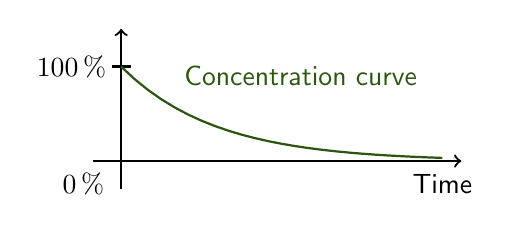
\begin{tikzpicture}[scale=1.2,thick]
    \draw[->](-3mm,0mm)--(36mm,0mm) node at (34mm,-2.4mm){Time};
    \node at (-4mm,-2.4mm){$0\,\%$};
    \draw[->](0mm,-3mm)--(0mm,14mm);
    \draw(-1mm,10mm)--(1mm,10mm) node[left=1.8mm]{$100\,\%$};
    \draw[color=mygreen,domain=0:3.4] plot(\x,{exp(-\x)});
    \node at (19mm,9mm){\mygreen{Concentration curve}};
  \end{tikzpicture}
\end{minipage}
\clearpage
%
% SLIDE 8 ----------------------------------------------------------
%
\section{Conclusion}
	\begin{enumerate}
		\item Give a conclusion, where you \mygreen{recall} the \mygreen{main points}!
		\item This also gives the snoring persons time to wake up!
	\end{enumerate}
\clearpage
%
% SLIDE 9 ----------------------------------------------------------
%
\thispagestyle{empty}
% background (stroke)
\begin{tikzpicture}[remember picture,overlay]
	\node [xshift=\paperwidth/2,yshift=\paperheight/2] at (current page.south west)[rectangle,fill,inner sep=0pt,minimum width=\paperwidth,minimum height=\paperheight/3,top color=mygreen,bottom color=mygreen]{};
\end{tikzpicture}%
% content
\begin{flushright}
	\vspace{0.6cm}
	\color{white}\sffamily
	{\bfseries\Large
	Questions?	
	\par}
	\vfill
%	\includegraphics[width=0.25\textwidth]{./contents/logo}%
\end{flushright}
% ------------------------------------------------------------------------------
% End document
% ------------------------------------------------------------------------------
\end{document}
